\documentclass[letterpaper]{article}
\DeclareSymbolFont{AMSb}{U}{msb}{m}{n}
\DeclareMathAlphabet{\mathbbm}{U}{bbm}{m}{n}

\title{Functors, Fixed Points, and Algebras; Oh My!}

\usepackage{amsmath,amssymb,amsthm,latexsym}
\usepackage{fancyhdr}
\usepackage[tiny,center,compact,sc]{titlesec}
\usepackage[cm]{fullpage}
\usepackage{pstricks}
\usepackage{graphicx}
\usepackage{verbatim}
\usepackage{bm}
\usepackage{ifthen}
\usepackage{epsfig}
\usepackage{tikz}
 \usetikzlibrary{arrows,calc,matrix,positioning,scopes}
\usepackage{textcomp}
\usepackage{url}
\usepackage{multirow}
\usepackage{hyperref}
\usepackage{listings}
  \lstloadlanguages{Haskell}
\usepackage{breakurl}

\renewcommand{\baselinestretch}{0.9}

%\newtheorem{thm}{Thm}[section]
%\newtheorem{dfn}{Def}[section]

\setlength{\parindent}{0pt}
\setlength{\parskip}{3pt}

%Scalable bracket-like
\newcommand{\paren}[1]{\left({#1}\right)}
\newcommand{\brak}[1]{\left[{#1}\right]}
\newcommand{\abs}[1]{\left\lvert{#1}\right\rvert}
\newcommand{\ang}[1]{\left\langle{#1}\right\rangle}
\newcommand{\set}[1]{\left\{#1\right\}}

%Mathematics
\newcommand{\condexp}[1]{\ifthenelse{\equal{#1}{false}}{}{^{#1}}}
\newcommand{\dd}[3][false]{\frac{d\condexp{#1}{#2}}{d{#3}\condexp{#1}}}
\newcommand{\pd}[3][false]{\frac{\partial\condexp{#1}{#2}}{\partial{#3}\condexp{#1}}}

\newcommand{\ifrac}[2]{{#1}/{#2}}

%Quantum Mechanics
\newcommand{\ket}[1]{\left\lvert{#1}\right\rangle}
\newcommand{\bra}[1]{\left\langle{#1}\right\rvert}
\newcommand{\braket}[2]{\left\langle{#1}\middle\vert{#2}\right\rangle}
\newcommand{\Braket}[3]{\left\langle{#1}\middle\vert{#2}\middle\vert{#3}\right\rangle}
\newcommand{\dyad}[2]{\left\lvert{#1}\middle\rangle\middle\langle{#2}\right\rvert}

\DeclareMathOperator{\mm}{\mid\mid}

\newcommand{\defn}[1]{{\bf #1}}

\begin{document}
\maketitle

For a given endofunctor $F : \mathcal{C} \to \mathcal{C}$, let
%
\begin{itemize}
%
  \item $(\mu F, in)$ denote its initial algebra ($in : F(\mu F) \to \mu F$)
  A {\em catamorphism} $h$ is the unique arrow from an initial algebra to
  any other $a$; it must be the solution to the equation $h \circ in = a
  \circ F h$.
%
  \item $(\nu F, out)$ denote its terminal coalgebra ($out : \nu F \to F(\nu
  F)$) An {\em anamorphism} of a coalgebra $c$ is the unique solution to $c
  \circ h = F h \circ out$.
%
\end{itemize}


\section{Special Fixed Points}

\subsection{Carrier of Initial Algebra Implies Fixed Point}

Assume that $(\mu F, in)$ exists; then $(F(\mu F), F(in))$ is also an
$F$-algebra (because $F(in) : F(F(\mu F)) \to F(\mu F)$) and the following
diagram exists in $\mathcal{C}$:
%
\begin{center}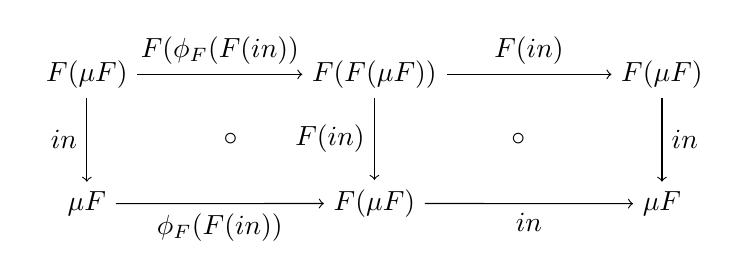
\begin{tikzpicture}

  \matrix (m) [matrix of math nodes, row sep=3em, column sep=6em]
  %
  { F(\mu F) & F(F(\mu F)) & F(\mu F) \\ \mu F & F(\mu F) & \mu F \\ };

  \path [->] (m-1-1) edge node [above] {$F(\phi_F(F(in))$} (m-1-2) ;

  \path [->] (m-1-2) edge node [above] {$F(in)$} (m-1-3) ;

  \path [->] (m-1-1) edge node [left] {$in$} (m-2-1) ;

  \path [->] (m-1-2) edge node [left] {$F(in)$} (m-2-2) ;

  \path [->] (m-2-1) edge node [below] {$\phi_F(F(in))$} (m-2-2) ;

  \path [->] (m-2-2) edge node [below] {$in$} (m-2-3) ;

  \path [->] (m-1-3) edge node [right] {$in$} (m-2-3) ;

  \node at ($(m-1-1)!0.5!(m-2-2)$) {$\circ$} ;

  \node at ($(m-1-2)!0.5!(m-2-3)$) {$\circ$} ;

\end{tikzpicture}\end{center}
%
where $\phi_F(F(in))$ is the catamorphism of $F(in)$: the unique arrow
guaranteed to exist by initiality of $(\mu F, in)$ such that the left square
commutes.  The right square trivially commutes and is rendered only for
convenience.  (Note that $\phi_F(in) = id$ by initiality!)

We see that $in \circ \phi_F(F(in))$ (the bottom two arrows of the diagram)
form an algebra homomorphism from $(\mu F, in)$ to itself.  By initiality,
this must be the identity: $in \circ \phi_f(F(in)) = 1_{\mu F}$.

The top-left and middle edges compose to give $F(in) \circ F(\phi_F(F(in))$,
which is just $F(in \circ \phi_F(F(in)))$ (because functors distribute over
compostion), which we know to be $F(1_{\mu F})$, which is $1_{F(\mu F)}$
(because functors send identity arrows to identity arrows).  By commutation
of the left square, the left and bottom-left arrows' composition,
$\phi_F(F(in)) \circ in = 1_{F(\mu F)}$.

All told, then, $in$ is an isomorphism with inverse $in^{-1} = \phi_F(F(in))$.
That is, $\mu F$ satisfies the equation $\mu F \simeq F(\mu F)$, so $\mu F$
is a fixed point of $F$.  (This is apparently known as ``Lambek's Lemma''.)

\subsection{Carrier of Final Coalgebra Implies Fixed Point}

The above argument dualizes in a straightforward way.
%
\begin{center}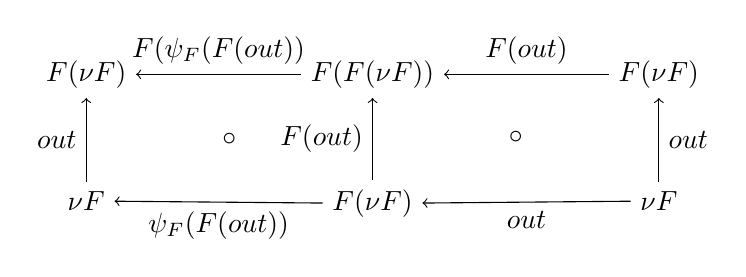
\begin{tikzpicture}

  \matrix (m) [matrix of math nodes, row sep=3em, column sep=6em]
  %
  { F(\nu F) & F(F(\nu F)) & F(\nu F) \\ \nu F & F(\nu F) & \nu F \\ };

  \path [<-] (m-1-1) edge node [above] {$F(\psi_F(F(out))$} (m-1-2) ;

  \path [<-] (m-1-2) edge node [above] {$F(out)$} (m-1-3) ;

  \path [<-] (m-1-1) edge node [left] {$out$} (m-2-1) ;

  \path [<-] (m-1-2) edge node [left] {$F(out)$} (m-2-2) ;

  \path [<-] (m-2-1) edge node [below] {$\psi_F(F(out))$} (m-2-2) ;

  \path [<-] (m-2-2) edge node [below] {$out$} (m-2-3) ;

  \path [<-] (m-1-3) edge node [right] {$out$} (m-2-3) ;

  \node at ($(m-1-1)!0.5!(m-2-2)$) {$\circ$} ;

  \node at ($(m-1-2)!0.5!(m-2-3)$) {$\circ$} ;

\end{tikzpicture}\end{center}
%
Where $\psi_F(F(out))$ is the anamorphism guaranteed by terminality of $(\nu
F, out)$.  $\psi_F(F(out)) \circ out = 1_{\nu F}$ by terminality (and
$\psi_F(out) = id$; also note that dualization has swapped which half of the
isomorphism follows immediately!).  In the other direction, $out \circ
\psi_F(F(out)) = F(\psi_F(F(out))) \circ F(out) = F(\psi_F(F(out)) \circ
out) = F(1_{\nu_F}) = 1_{F(\nu_F)}$.

Thus $out$ is an isomorphism with inverse $out^{-1} = \psi_F(F(out))$ and
$\nu_F$ satisfies $\nu_F \simeq F(\nu F)$, making it another fixed point.

\subsection{Other Fixed Points}

We know that {\em any} fixed point of $F$ in fact, call it $\theta F$, has
the property of being isomorphic to $F(\theta F)$.

\subsubsection{An Example or Two of Fixed Points}

For the purpose of this section, consider the lovely binary tree functor on
the category $\mathbf{Set}$, which has (countable) (co)products, initial
object $\emptyset$ and terminal object $1$; i.e., $T x = 1 + x \times x$.
Then,
%
\begin{itemize}
%
  \item One fixed point, in fact the smallest, of $F$ is the collection of
  {\em finite} binary trees with $1$ at its leaves.  This is the usual thing
  obtained by inflation.
%
  \item The largest is binary trees with {\em countable} (including finite)
  paths (and $1$ leaves).  This cannot be defined by inflation but is
  clearly closed under $T$: taking the product of two such such objects is
  clearly another such object.
%
  \item Another intermediate structure $\theta T$ is less obvious: trees
  which may descend {\em left} countably many times but {\em right} only
  finitely many times.  Again, we cannot grow this by inflation but can
  argue that the product of any two such objects is, indeed, another such
  object.
%
\end{itemize}
%
Note that, indeed, as we might expect, $\mu T \subsetneq \theta T \subsetneq
\nu T$.  The ``other $\theta T$'' (which swaps left and right) is also
between $\mu T$ and $\nu T$, but is not comparable to $\theta T$: fixed
points form a partial order with a single bottom and single top.

Consider a different functor, the diagonal product functor $\Delta x = x
\times x$, which is like $T$ except that it omits the ``$1 +$'' part.  In
this case,
%
\begin{itemize}
%
  \item $\mu \Delta = \emptyset$.  There's nothing to force us away and
  $\Delta \emptyset = \emptyset \times \emptyset \simeq \emptyset$.
%
  \item The terminal object $1$ is $\nu \Delta$: $\Delta 1 = 1 \times 1
  \simeq 1$.  For ease of understanding, this is the singleton set whose
  element represents a tree that is its own root's left and right child.
%
  \item There are no other fixed points of $\Delta$.  (Stated without
  proof!)
%
\end{itemize}
%
As before, $\mu \Delta \subseteq \nu \Delta$.

\subsection{Induced Duals}

Because of the two isomorphisms above, we know that $(\mu F, \phi_F(F(in))) =
(\mu F, in^{-1})$ exists and is a coalgebra; similarly, $(\nu F,
\psi_F(F(out))) = (\nu F, out^{-1})$ exists and is an algebra.  That is, we
have these diagrams (on the left are $F$-algebras and on the right are
$F$-coalgebras; both diagrams take place in $\mathcal{C}$):
%
\begin{center}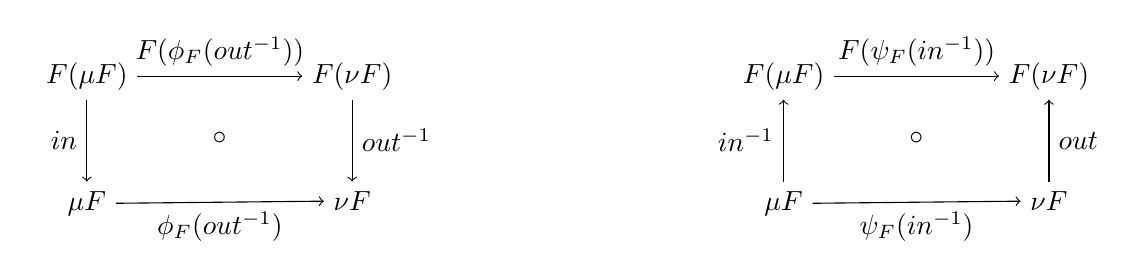
\begin{tikzpicture}

  \matrix (m) [matrix of math nodes, row sep=3em, column sep=6em]
  %
  { F(\mu F) & F(\nu F) & & F(\mu F) & F(\nu F) \\
    \mu F & \nu F & & \mu F & \nu F \\ } ;

  \path [->] (m-1-1) edge node [left] {$in$} (m-2-1) ;
  \path [->] (m-1-2) edge node [right] {$out^{-1}$} (m-2-2) ;
  \path [->] (m-2-1) edge node [below] {$\phi_F(out^{-1})$} (m-2-2) ;
  \path [->] (m-1-1) edge node [above] {$F(\phi_F(out^{-1}))$} (m-1-2) ;
  \node at ($(m-1-1)!0.5!(m-2-2)$) {$\circ$} ;

  \path [->] (m-2-4) edge node [left] {$in^{-1}$} (m-1-4) ;
  \path [->] (m-2-5) edge node [right] {$out$} (m-1-5) ;
  \path [->] (m-2-4) edge node [below] {$\psi_F(in^{-1})$} (m-2-5) ;
  \path [->] (m-1-4) edge node [above] {$F(\psi_F(in^{-1}))$} (m-1-5) ;
  \node at ($(m-1-4)!0.5!(m-2-5)$) {$\circ$} ;

\end{tikzpicture}\end{center}
%
where, again, $\phi_F(out^{-1}) = \phi_F(\psi_F(F(out)))$ is the unique arrow that
makes the diagram commute, guaranteed to exist by initiality of $(\mu F,
in)$ and, dually, $\psi_F(\phi_F(F(in))) = \psi_F(in^{-1})$ by terminality of
$(\nu F, out)$.  Note that this existence argument does {\em not} make these
arrows equal.

\subsubsection{Example Induced Coalegbra}

For this section, we're going to write fuctions in Haskell, though only for
its syntax.  Please read all definitions as strict and total!

Consider the List (of $A$s) $\mathbf{Set}$ endo-functor $ListF~x = 1 + A \times
x$.  Let's give it a Haskell rendering, choosing $A = \text{Int}$ just to
dodge polymorphism:
%
\begin{lstlisting}[language=Haskell]
data ListF rec = FNil | FCons Int rec
\end{lstlisting}
%
$\mu L$ is (isomorphic to) the traditional \textsc{lisp}-y lists whose
elements are of type $A$:
%
\begin{lstlisting}[language=Haskell]
data MuListF = MLNil | MLCons Int MuListF
\end{lstlisting}
%
$in : L (\mu L) \to \mu L$ sends $1$ to the empty
list and $a \times l$ to the list whose head is $a$ and tail is $l$:
%
\begin{lstlisting}[language=Haskell]
_in :: ListF MuListF -> MuListF
_in FNil = MLNil
_in (FCons i l) = MLCons i l
\end{lstlisting}
%
Moreover, we know (stated without proof) that $L$'s catamorphism is an
uncurried foldr: looking at the type, we see $\phi_L : \forall_X . (L X \to
X) \to (\mu L \to X)$.  (Expanding things a bit, this is $\forall_X . ((1 +
A \times X) \to X) \to \mu L \to X$ which is iso to $\forall_X . (A \to X
\to X) \to X \to \mu L \to X$.)  In particular, it is
%
\begin{lstlisting}[language=Haskell]
phiL :: forall a . (ListF a -> a) -> MuListF -> a
phiL f MLNil = f (FNil)
phiL f (MLCons i l) = f (FCons i (phiL f l))
\end{lstlisting}
%
As required, $\phi_L(in) = id$:
%
\begin{lstlisting}[language=Haskell]
phiL _in MLNil = _in FNil = MLNil

phiL _in (MLCons i l)
  = _in (FCons i (phiL f l))
  = _in (FCons i l)	-- induction
  = MLCons i l
\end{lstlisting}
%
$in^{-1} = \phi_L(L(in))$ instantiates $\phi_L$ with $X = L (\mu L)$.  The
function $L(in) : L (L \mu L) \to L \mu L$ then is just \texttt{fmap in}.
So $in^{-1} = \phi_L(L(in)) : \mu L \to L \mu L$ is
\begin{lstlisting}[language=Haskell]
phiL (fmap _in) MLNil = (fmap _in) FNil = FNil

phiL (fmap _in) (MLCons i l)
  = (fmap _in) (FCons i (phiL (fmap _in) l))
  = FCons i (_in (phiL (fmap _in) l))
  = FCons i l
\end{lstlisting}

\subsubsection{Example Induced Algebra}

$\nu L$ is the set of possibly-infinite lists: it contains all of $\mu L$ as
well as the non-terminating lists.  $out$ sends nil to the left $1$ and a
list with cons cell top to the right product of its head and tail.  So what
is $\psi_L$?  We know from looking at the diagram that it must have type
$\forall_X . (X \to L X) \to X \to \nu L$.

\end{document}
